\subsection*{ตัวอย่างชุดข้อมูลสำหรับการทดสอบโมเดลปัญญาประดิษฐ์ในการตรวจจับภาพบุคคล}
\begin{figure}[!ht]
    \centering
   \begin{subfigure}[b]{0.55\linewidth}
      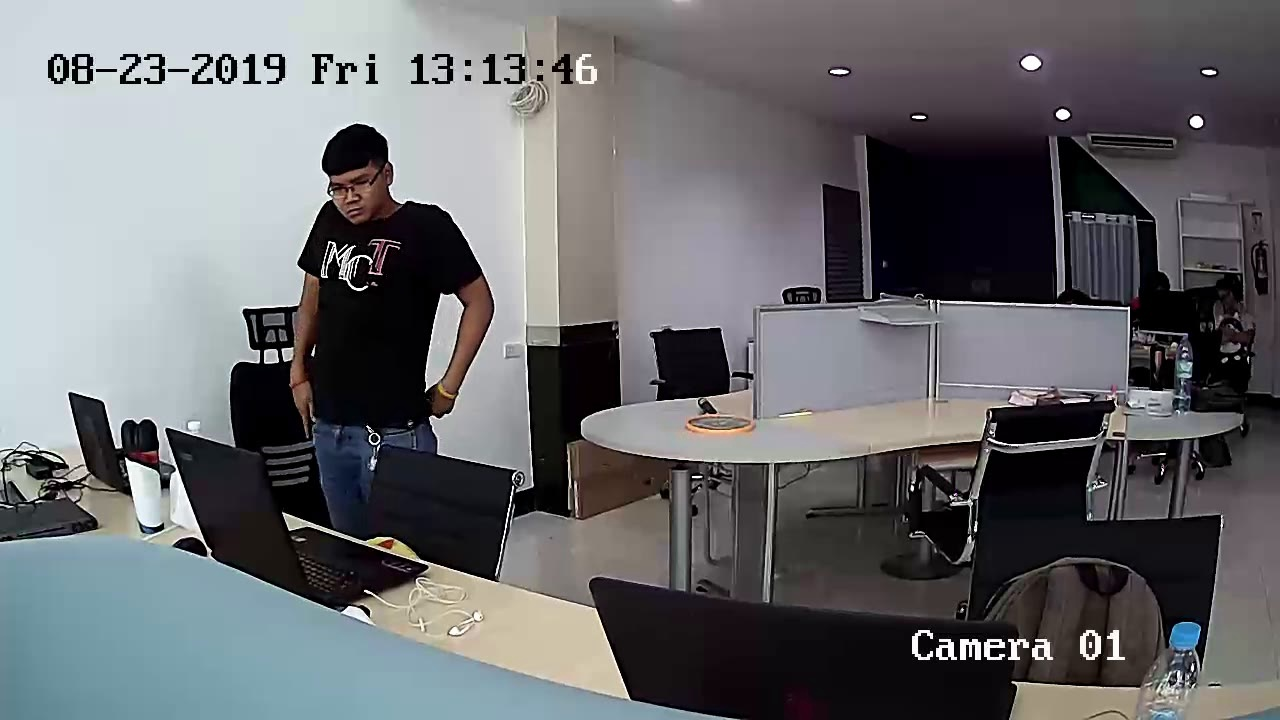
\includegraphics[width=\linewidth]{appendix/images/3.jpg}
    \end{subfigure}
    \begin{subfigure}[b]{0.55\linewidth}
      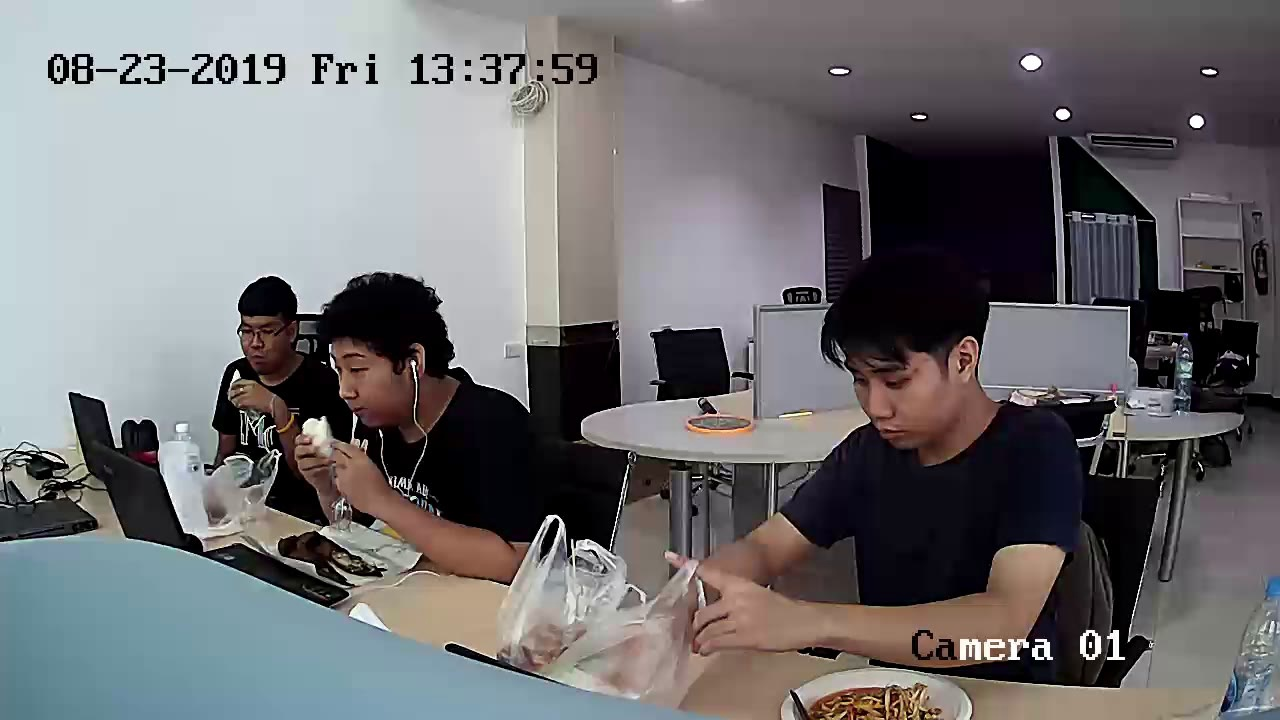
\includegraphics[width=\linewidth]{appendix/images/5.jpg}
    \end{subfigure}
    \begin{subfigure}[b]{0.55\linewidth}
      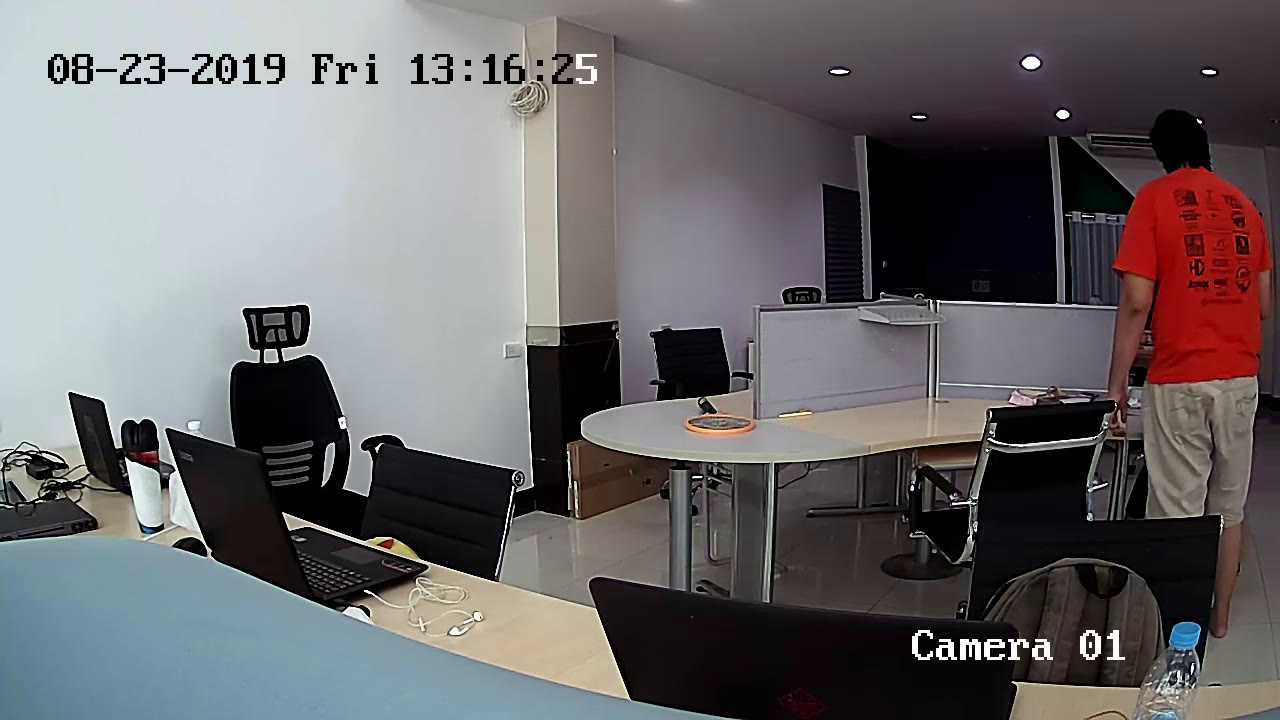
\includegraphics[width=\linewidth]{appendix/images/8.jpg}
    \end{subfigure}
    \begin{subfigure}[b]{0.55\linewidth}
      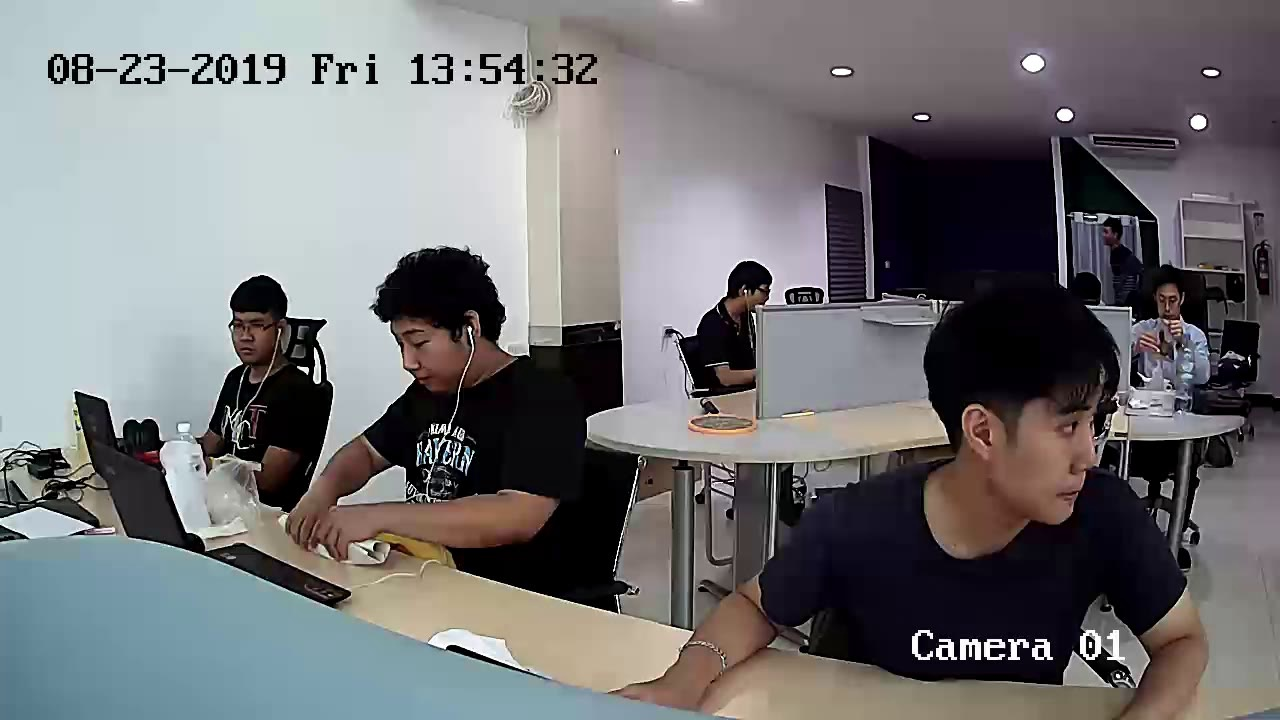
\includegraphics[width=\linewidth]{appendix/images/17.jpg}
    \end{subfigure}
    \caption{รูปผลลัพธ์การทำงานของหน้าต่าง Track}
    \label{fig:result_track}
  \end{figure}
